\documentclass[a4j,10pt,onecolumn]{ujarticle} % jsbook, jsreportなど

%% マージン等の設定
%% A4: 210 x 297 mm
%% jsクラスではフォントサイズを10ptから変更するときには長さ単位にtrueをつける必要がある.
%% inch->trueinch, mm->truemm, cm->truecmなど.
\setlength{\textwidth}{15truecm}       %% 150mm + 1inch(25.4mm)*2 + 4.6mm*2 = 210mm
\setlength{\oddsidemargin}{4.6truemm}  %% 左右余白30mm
\setlength{\evensidemargin}{4.6truemm}
\setlength{\textheight}{227truemm} %% 227mm + 1inch*2 + 9.6mm*2 = 297mm
\setlength{\headheight}{9.6truemm} %% 上下余白35mm
\setlength{\topmargin}{9.6truemm}
\setlength{\headsep}{-15truemm}
\setcounter{secnumdepth}{4}
%% 代わりに以下2行でもOK
%% \usepackage{geometry}
%% \geometry{top=35truemm,bottom=35truemm,left=30truemm,right=30truemm}

%% \renewcommand{\baselinestretch}{0.82}

%% 使いたいパッケージを指定
\usepackage[dvipdfmx]{graphicx, color} % 画像挿入
\usepackage{mediabb} % PDFなどのbounding boxを取得してくれる
\usepackage{amsmath} % 数式用パッケージ
\usepackage{url} % URL挿入用
\usepackage{color} % 文字色指定
\usepackage{bm} % bold math (数式中のベクトルなどで太字にしたいとき)
\usepackage{titlesec}
\usepackage{listings}

% コード読み込みのための設定
\lstset{%
  tabsize=8,
  language={Python},
  basicstyle={\small},%
  identifierstyle={\small},%
  commentstyle={\small\itshape},%
  keywordstyle={\small\bfseries},%
  ndkeywordstyle={\small},%
  stringstyle={\small\ttfamily},
  frame={tb},
  breaklines=true,
  columns=[l]{fullflexible},%
  numbers=left,%
  xrightmargin=0zw,%
  xleftmargin=3zw,%
  numberstyle={\scriptsize},%
  stepnumber=1,
  numbersep=1zw,%
  lineskip=-0.2ex,%
  showstringspaces=false
}

%% マクロ(ユーザ定義命令)を宣言
\newcommand{\hoge}{\textcolor{red}{ほげほげ}}    % 引数なし
\newcommand{\Hoge}[2]{\textcolor{#1}{#2#2}}      % 引数あり
\newcommand{\HOGE}[2][red]{\textcolor{#1}{#2#2}} % 引数あり(オプション引数付き)

\makeatletter

\def\@thesis{卒業論文}
\def\@professor{神崎亮平}
\def\id#1{\def\@id{#1}}
\def\department#1{\def\@department{#1}}

\def\@maketitle{
\begin{center}
{\huge \@thesis \par} %修士論文と記載される部分
\vspace{10mm}
{\LARGE\bf \@title \par}% 論文のタイトル部分
\vspace{10mm}
{\Large \@date 提出\par}	% 提出年月日部分
\vspace{20mm}
{\Large 指導教員 \@professor 教授\par} % 指導教員
\vspace{20mm}
{\Large \@department \par}	% 所属部分
% {\Large 学籍番号 \@id \par}	% 学籍番号部分
\vspace{10mm}
{\large \@id \@author}% 氏名
\end{center}
\par\vskip 1.5em
}

\makeatother

\title{\underline{神経回路シミュレーションにおける}\\\underline{イオンチャンネルダイナミクス計算の}\\\underline{最適化コードの自動生成}}
\date{\today}
\department{東京大学工学部機械情報工学科}
\id{03-150268}
\author{井上裕太}

%% --- 以下本文 ---
\begin{document}
\maketitle %% タイトルを表示

% \chapter{チャプター}
% jsarticleには\verb+\chapter+命令がない.

%% 目次作成
\clearpage
\tableofcontents
\clearpage
\listoffigures
\clearpage
\listoftables

% \section{序論}
\subsection{研究の背景}
脳機能の理解を目的として,スーパコンピュータを用いた神経回路のシミュレーションが行われている. また,消費電力やシミュレーションの割り当て時間といったリソースの問題やリアルタイムデータ同化への需要から
シミュレーションの高速化・最適化が求められている. しかし,神経細胞には様々な種類のものが存在するため,個々の神経細胞のイオンチャンネルのモデルを最適化された形で実装するために,これまでそれぞれのモデルに対して多大な努力が行われてきた.
また,現代の計算機にも多様な種類が存在し,それぞれに対する最適化も個別に行われてきた.
本研究の目的はそれぞれの細胞モデルのシミュレーションコードを個々のアーキテクチャに合わせて,自動又は半自動的に最適化を行う手法を確立することである.

\subsection{研究の目的と手法}
通常はソース内で
何回改行しようと
このように
出力
結果で改行は
起こらない.
改行するには\\
\verb+\+\verb+\+や\verb+\newline+を用いる.

また,このようにソースで一行空けると
改段落が発生する.自動的に字下げされているよね.\verb+\par+でも同じ.\par
字下げを明示的に指定するには\verb+\indent+や\verb+\noindent+を使う.

\noindent このようにインデントが抑制される.

\verb+\newpage+をというコマンドもあり,使うと{\newpage}こうなる.

\subsection{本論文の構成}
本論文は全5章から構成される.
本章では本研究の背景・目的について述べた.
第2章では,実験方法について述べる.

\clearpage
\section{数式}
\subsection{挿入方法}
{\TeX}の大きな特徴は綺麗な数式.
挿入方法には文中に入れる方法と別の行にセンタリングして入れる方法がある.
文中に数式を入れたかったら,は\verb+$y=f(x)$+($y=f(x)$)のように\verb+$+にはさむ.
別行に表示したかったらequation環境かeqnarray環境を使えばよい.
eqnarray環境は複数行の数式を位置を揃えて記述したい場合に用いる.
equation環境だと
\begin{equation}
  y=f(x)
\end{equation}
こうなり,
eqnarray環境だと
\begin{eqnarray}
  y&=&f(x)     \label{eq:func} \\
  &=&x^2-3x+1  \label{eq:polynominal}
\end{eqnarray}
こうなる.eqnarray環境中の\verb+&+マークは揃えたい位置の指定に用いる(=をはさめば=でそろう).
また,もし式(\ref{eq:func}),(\ref{eq:polynominal})のように番号をつけたくなければ,\verb+\nonumber+かeqnarray*環境を用いる.
\begin{eqnarray}
  y&=&f(x) \nonumber \\
  &=&x^2-3x+1
\end{eqnarray}
\begin{eqnarray*}
  y&=&f(x) \\
  &=&x^2-3x+1
\end{eqnarray*}

\subsection{色々な数式}
様々な記号・記法があるので詳しくはググっていただきたいが,少しだけ紹介する.

\noindent \textbf{記号} \
\verb+$\alpha$+ $\rightarrow$ $\alpha$,\verb+$\theta$+ $\rightarrow$ $\theta$,
\verb+$\Theta$+ $\rightarrow$ $\Theta$,\verb+$\infty$+ $\rightarrow$  $\infty$

\noindent \textbf{分数} \
\verb+$\frac{A}{B}$+ $\rightarrow$
\begin{equation*}
  \frac{A}{B}
\end{equation*}

\noindent \textbf{括弧} \
\verb+\left(, \right), \left[, \right]+など.高さも調節してくれる.
\begin{equation*}
  f(x)=\left \{ \begin{array}{l}
    1 \ (x=1のとき) \\
    0 \ (x\neq1のとき)
  \end{array}
  \right.
\end{equation*}

\begin{flushleft}
\noindent \textbf{文字装飾} \
\verb+$x^{2a}$+ $\rightarrow$ $x^{2a}$,
\verb+$x_{2b}$+ $\rightarrow$ $x_{2b}$,
\verb+$\overline{g}$+ $\rightarrow$ $\overline{g}$,
\verb+$\underline{g}$+ $\rightarrow$ $\underline{g}$,
\verb+${\bm y}=A{\bm x}$+ $\rightarrow$ ${\bm y}=A{\bm x}$(bm.styを使用)
\end{flushleft}

\noindent \textbf{斜体にしない文字} \
\verb+${\rm sin}$+ $\rightarrow$ ${\rm sin}$
または
\verb+$\sin$+ $\rightarrow$ $\sin$

\noindent \textbf{総和} \
\verb+$S_n=\sum_{k=1}^{n}(x_k)^2$+ $\rightarrow$
\begin{equation*}
  S_n=\sum_{k=1}^{n}(x_k)^2
\end{equation*}

\clearpage
\section{シミュレーションのモデルと環境}
% シミュレーションを行ったモデル
\subsection{シミュレーションモデル}
本研究では,先行研究として触れた宮本\cite{miyamoto-master}\cite{miyamoto-master-eng}らが手動で行った最適化を自動で行うことを目的としている.
そのため, 最適化の対象となるシミュレーションモデルに同じものを採用した.
% HHモデル
\subsubsection{Hodgkin-Huxleyモデル}
\cite{Hodgkin1990}


% pasモデル
\subsubsection{Pasモデル}

( TODO : 時間がなければ消す or 付録としてくっつける)


% シミュレーションを行うソフトウェアについて
\subsection{シミュレータ}
NEURONは,Yale大学のHinesらによって開発されている神経回路・細胞シミュレーションソフトウェアであり,
神経回路シミュレーションにおいて標準の一つとなっており,先行研究としてあげた宮本らによる
手動での高速化においても対象となったソフトウェアである. そのため,本研究の目的である神経回路シミュレーションの自動最適化の
対象としてNEURONを採用した. また,京やクラスタといった複数の計算機上で安定して稼働させるためにNEURONのバージョンは7.2を選択した.\\

\subsubsection{全体構成}
NEURONでは,MODファイルとHOCファイルと呼ばれる二つのファイルに必要な情報を記述することで神経回路シミュレーションを行っている.\\
MODファイルはその名のとおり神経細胞のモデルを記述するファイルであり, ( TODO : 章番号)で示したように神経細胞を数理モデルとして記述する.\\
一方でHOCファイルと呼ばれるファイルにはMODファイルで記述された神経細胞モデル間のつながりや,
シミュレーション時間などシミュレーションそのものに関与する設定を記述する.\\
より具体的には,図 ( TODO: 番号)で示したように,nrnivmodlと呼ばれるトランスパイラによってMODファイルは対応するCファイルに変換される.
このCファイルはさらにGCCやICCといったC言語のコンパイラによってオブジェクトファイルになり,ここで生成されたオブジェクトファイルと
NEURON本体がリンクされることによってNEURONの実行形式が作成されることになる.
そのため,MODファイルとして利用者が作成したモデルは実行時にはNEURONに組み込まれていることとなる.\\
最終的にこうして生成されたNEURONの実行形式に対してシミュレーションの情報を記述したHOCファイルを渡すことでシミュレーションが実行される.\\
\begin{figure}[htb]
% h:here, t:top, b:bottom, p:page
  \begin{center}
    \includegraphics[width=10.0cm, angle=-90]{./images/neuron}
    \caption{NEURONの全体構成}
    \label{fig:neuron}
  \end{center}
\end{figure}~\\
宮本らによる先行研究では,主にこのMODファイルからCファイルへの変換に着目し,nrnivmodlによって作成されたCファイルを手動にて
最適化することでシミュレーション全体の高速化を達成した.\\
そのため,本研究においてはnrnivmodlに変わるトランスパイラを作成し自動での高速化を図る.\\

\subsubsection{NEURONのコンパイル}
\paragraph{クラスタ上でのコンパイル}~\\
クラスタのようなx86の大規模計算機では,
{\footnotesize
\begin{lstlisting}[caption=クラスタでのNEURONのコンパイル,label=cluster-neuron-compile,numbers=none]
$ ./configure --prefix=`pwd`\
              --without-iv --without-x --without-nrnoc-x11
$ make
$ make install
\end{lstlisting}
}
とすることで計算シミュレータとしてのNEURONをコンパイルし,実行形式を得ることができる.
デフォルトのコンパイルオプションではNEURONはGUI関係のライブラリもリンクするが,大規模計算機環境上では必要ないためオプションを渡すことで
コンパイル対象から除外している.\\
\paragraph{京上でのコンパイル}~\\
一方で,京ではログインノードと呼ばれるNEURONのコンパイルを行う環境(x86)とプログラムを実行する環境(sparc64)が
異なるため,クロスコンパイルを行う必要がある.\\
NEURONのコンパイルは内部的には\\
1. MODコンパイラ(nmodl)をコンパイルし実行形式を生成\\
2. MODコンパイラがMODファイルをC言語ファイルに変換した上でコンパイル\\
3. NEURON本体(nrniv, nrnoc)をコンパイルする\\
4. 上述の2と3をリンクさせ,実行形式を作成\\
という手順を踏んでいるが,この中でMODコンパイラ作成についてはログインノード(x86)で実行する必要があるため,1について
ネイティブコンパイルで,2,3,4についてはクロスコンパイルで行う必要がある.\\
またGUI関係のライブラリについてはクラスタ同様京でも必要ないため除外する(宮本 修論より引用)\\
\subparagraph{nmodlのコンパイル}~\\
{\footnotesize
\begin{lstlisting}[caption=京でのnmodlのコンパイル,label=k-nmodl-compile,numbers=none]
$ ./configure --prefix=`pwd`\
              --without-iv --without-x --without-nrnoc-x11\
              --with-nmodl-only linux_nrnmech=no\
              CC=gcc CXX=g++
$ make
$ make install
\end{lstlisting}
}
\subparagraph{NEURONのクロスコンパイル}~\\
NEURON本体をクロスコンパイルする前に, 上述したnmodlのコンパイルで生成した実行形式をPATHの通っているディレクトリに
移動させておく必要がある. nmodlを退避させたのち,下記のコマンドを実行することでNEURON本体の実行形式が生成される
{\footnotesize
\begin{lstlisting}[caption=京でのNEURON本体のコンパイル,label=k-neuron-compile,numbers=none]
$ make clean
$ ./configure --prefix=`pwd`\
              --without-x --without-nmodl\
              --host=sparc64-unknown-linux-gnu --build=x86_64-unknown-linux-gnu\
              --without-iv --without-nrnoc-x11\
              --enable-shared=no --enable-static=yes\
              --with-paranrn --with-mpi --with-multisend\
              linux_nrnmech=no use_pthread=no\
              CC=mpifccpx CXX=mpiFCCpx MPICC=mpifccpx MPICXX=mpiFCCpx
$ make
$ make install
\end{lstlisting}
}

\subsubsection{NMODLについて}
本研究ではMODファイルを変換する

% シミュレーションを行う環境について
\vspace{10cm}
\subsection{シミュレーション環境}
\subsubsection{計算機性能}
本研究で使用した計算機は,スーパーコンピュータ「京」(以下京, 図\ref{fig:k})と
研究室クラスタ(以下クラスタ, 図\ref{fig:cluster})である. 京はおよそ1京FLOPS(10PFLOPS)の演算性能をもち, 2011年の6月と11月にはTOP500\cite{top500}で世界第1位を,
2017年11月時点では世界第10位を記録している.\\
京の性能諸元\cite{riken-system}を表\ref{table:k}, \ref{table:k-processor}に, クラスタの性能諸元\cite{intel-xeon}を表\ref{table:cluster}に記す.\\

\begin{figure}[htb]
% h:here, t:top, b:bottom, p:page
  \begin{center}
    \includegraphics[width=10.0cm, angle=-90]{./images/k}
    \caption{スーパーコンピュータ京(提供: 理化学研究所)}
    \label{fig:k}
  \end{center}
\end{figure}~\\

\begin{table}[htb]
  \begin{center}
    \caption{京計算ノード構成}
    \begin{tabular}{|p{4cm}|p{10cm}|}
      \hline
      ピーク演算性能 & 10.62PFLOPS \\ \hline
      メモリ総容量 & 1.26PB(ノードあたり16GB)\\ \hline
      計算ノード間ネットワーク & 6次元メッシュ/トーラス(ユーザービューは3次元トーラス)\\ \hline
      帯域 & 3次元の正負各方向にそれぞれ5GB/s×2(双方向)\\ \hline
    \end{tabular}
    \label{table:k}
  \end{center}
\end{table}~\\

\vspace{2cm}
\begin{table}[ht]
  \begin{center}
    \caption{京プロセッサ構成}
    \begin{tabular}{|p{6cm}|p{8cm}|}
      \hline
      CPU性能 & 128GFLOPS(16GFLOPS×8コア)\\ \hline
      コア数 & 8個\\ \hline
      浮動小数点演算器構成(コアあたり)& 積和演算器: 4(2×2個 SIMD), (逆数近似命令: SIMD 動作)除算器: 2個 比較器: 2個\\
      & 浮動小数点レジスタ(64ビット): 256本 グローバルレジスタ(64ビット): 188本\\ \hline
      キャッシュ構成 & 1次命令キャッシュ: 32KB(2way), 1次データキャッシュ: 32KB(2-way), 2次キャッシュ: 6MB(12-way) コア間共有\\ \hline
      メモリ帯域 & 64GB/s(理論ピーク値)\\ \hline
      動作周波数 & 2GHz \\ \hline
      ダイサイズ & 22.7mm × 22.6mm \\ \hline
      トランジスタ数 & 約7億6000万個 \\ \hline
      消費電力 & 58W(プロセス条件TYP)\\ \hline
    \end{tabular}
    \label{table:k-processor}
  \end{center}
\end{table}~\\
\clearpage

\begin{figure}[h]
% h:here, t:top, b:bottom, p:page
  \begin{center}
    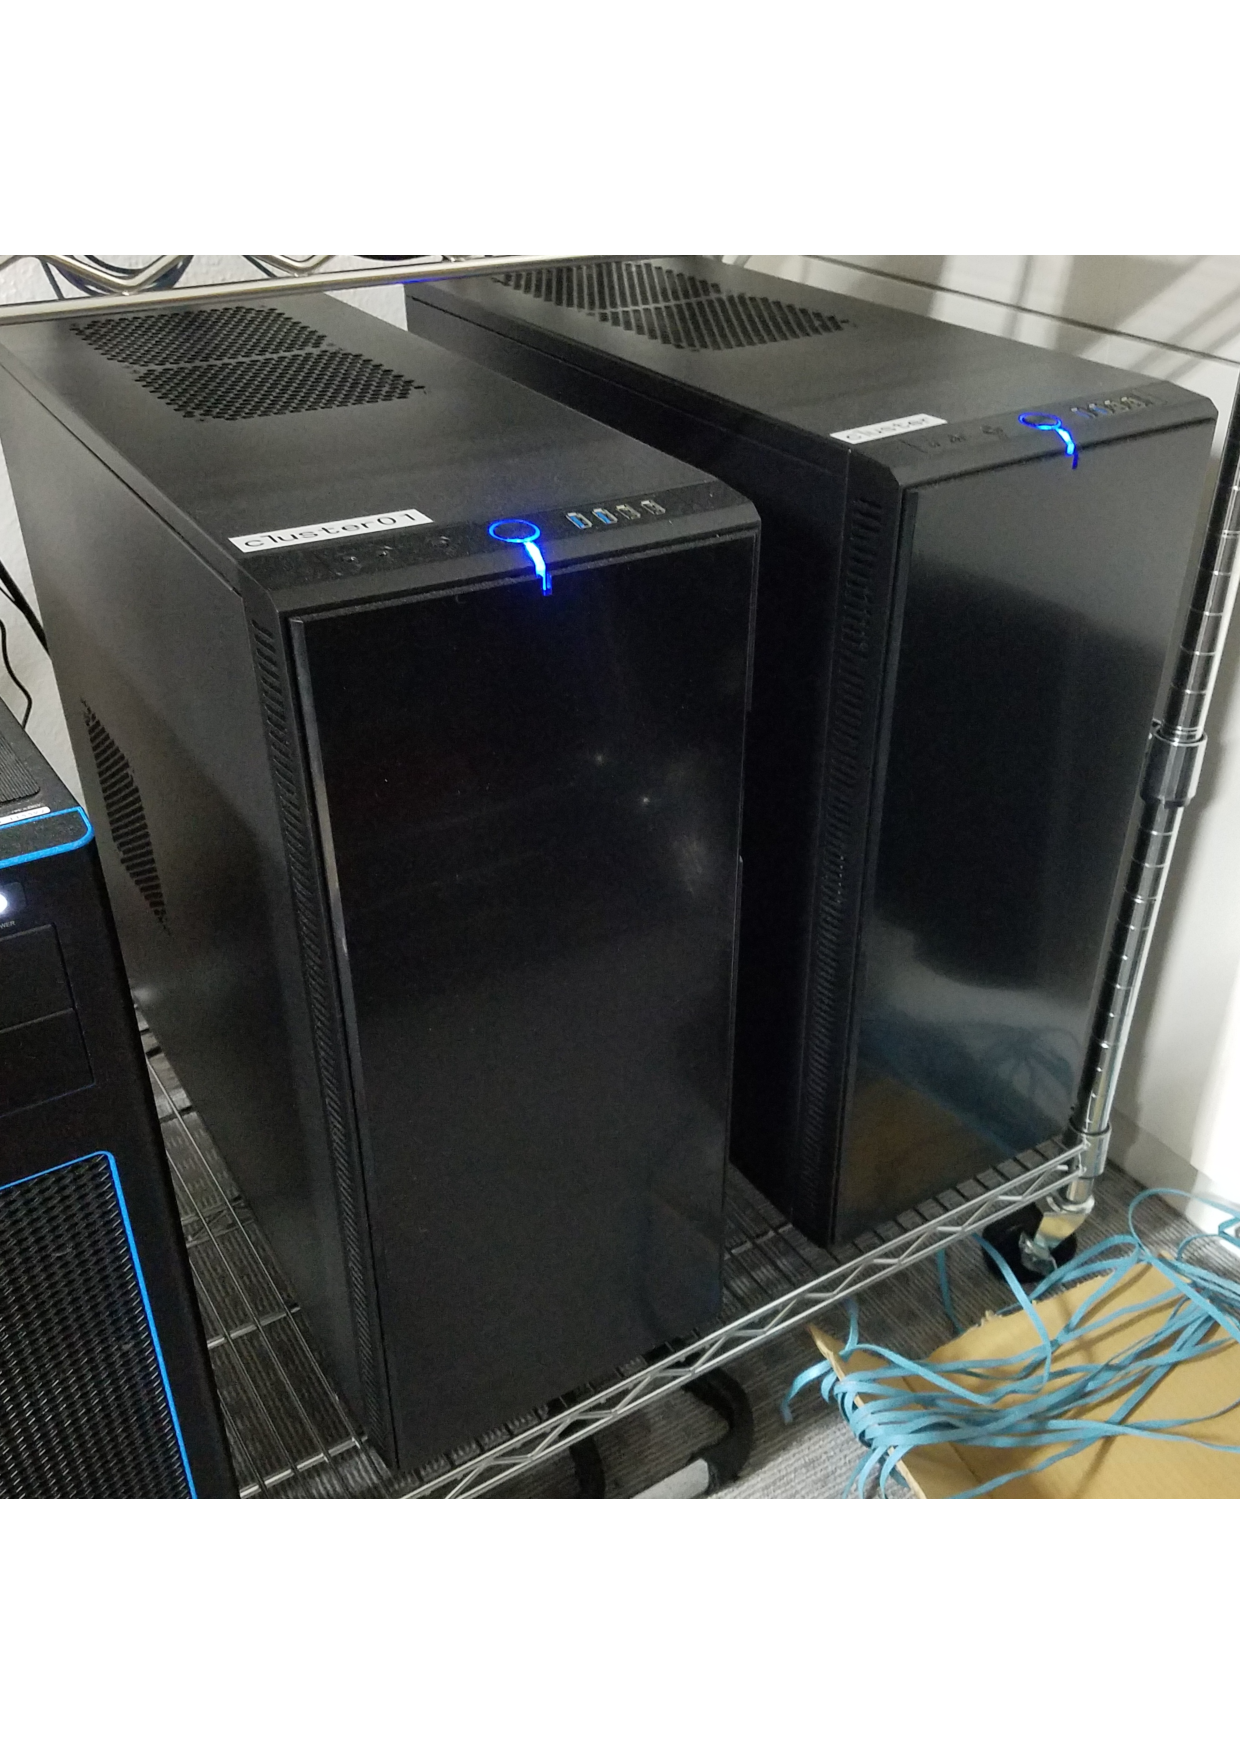
\includegraphics[width=8.0cm]{./images/cluster.pdf}
  \vspace*{-15mm}
  \caption{研究室クラスタ}
  \end{center}
  \label{fig:cluster}
\end{figure}~\\

\begin{table}[hb]
  \caption{クラスタ性能}
  \begin{center}
    \begin{tabular}{|p{4cm}|p{10cm}|}
      \hline
      CPU性能 & 268\.8 GFLOPS(19.2GFLOPS×14コア)\\ \hline
      コア数 & 14コア \\ \hline
      キャッシュ構成 & 1次命令キャッシュ: 448KB(2way), 1次データキャッシュ: 448KB(2-way), 2次キャッシュ: 3.5MB(12-way) コア間共有\\ \hline
      メモリ帯域 & 76.8GB/s(理論ピーク値)\\ \hline
      動作周波数 & 2.4GHz \\ \hline
      消費電力 & 120W\\ \hline
    \end{tabular}
    \label{table:cluster}
  \end{center}
\end{table}~\\

\clearpage
\subsubsection{ジョブ実行環境}
\label{subsec:job-env}
京に代表される大型コンピュータの場合,複数の利用者が共同で利用することが基本となる. そのため各個人が
各々勝手にプログラムを実行すると,計算が集中することで処理限界を大幅に超えてしまったり,逆に全く利用されない時間
などが現れてしまい計算資源を有効に活用できない. 従って, 大型コンピュータではキューイングシステムを利用してプログラムが実行される.\\
キューイングシステムにおける一度のプログラム実行の単位はジョブと呼ばれ,プログラムを実行する際に必要なノード数,メモリ,実行するプログラムのパスや前処理
といった情報を書き込んだジョブスクリプトを作成し,キューイングシステムにジョブスクリプトをサブミットすることでプログラムが実行される.\\
% clusterの説明
\paragraph{クラスタでのジョブの実行}~\\
\begin{table}[htb]
  \caption {クラスタでのジョブ関連コマンド}
  \begin{center}
    \begin{tabular}{|c|p{12cm}|}
      \hline
      コマンド & 説明 \\ \hline
      qsub & qsub \"サブミットするスクリプトのパス\"とすることでジョブをキューシステムに登録し,ジョブIDを出力する.\\ \hline
      qdel & pjdel \"ジョブID\"とすることで現在実行中または待機中のジョブを停止・削除する.\\ \hline
      qstat & 現在実行または待機中のジョブの一覧を表示する\\ \hline
    \end{tabular}
  \end{center}
\end{table}
\clearpage

{\footnotesize
\lstinputlisting[caption=クラスタのジョブスクリプト例, label=cluster-job-script,frame=single]{src/job/cluster-job}
}

{\footnotesize
\begin{lstlisting}[caption=クラスタでのコマンド実行例,label=cluster-job-example,numbers=none]
$ qsub job.sh
20252.cluster.localdomain

$ qstat
>> qstat
Every 1.0s: qstat                                                                                                                                            Wed Jan 10 01:06:06 2018

Job ID                    Name             User            Time Use S Queue
------------------------- ---------------- --------------- -------- - -----
20251.cluster              job.sh        inoue           00:05:38 C cluster
20252.cluster              job.sh        inoue                  0 R cluster
\end{lstlisting}
}

\begin{table}[htb]
  \caption {クラスタでのジョブの状態}
  \begin{center}
    \begin{tabular}{|c|p{12cm}|}
      \hline
      ジョブのステータス & 説明 \\ \hline
      Q & ジョブキューで待機中.\\ \hline
      R & ジョブを実行してる.\\ \hline
      C & ジョブが完了した.\\ \hline
    \end{tabular}
  \end{center}
\end{table}


% kの説明
\paragraph{京でのジョブの実行}~\\
\begin{table}[htb]
  \caption {京でのジョブ関連コマンド}
  \begin{center}
    \begin{tabular}{|c|p{12cm}|}
      \hline
      コマンド & 説明 \\ \hline
      pjsub & pjsub サブミットするスクリプトのパス\\
            & とすることでジョブをキューシステムに登録し,ジョブIDを出力する.\\ \hline
      pjdel & pjdel ジョブID\\
            & とすることで現在実行中または待機中のジョブを停止・削除する.\\ \hline
      pjstat & 現在実行または待機中のジョブの一覧を表示する\\ \hline
    \end{tabular}
  \end{center}
\end{table}

{\footnotesize
\lstinputlisting[caption=京のジョブスクリプト例, label=k-job-script,frame=single]{src/job/k-job}
}

\begin{table}[htb]
  \caption {京でのコマンド実行例}
{\scriptsize
\begin{framed}
\begin{verbatim}
$ pjsub job.sh
[INFO] PJM 0000 pjsub Job 7129316 submitted.

$ pjstat
ACCEPT QUEUED  STGIN  READY RUNNING RUNOUT STGOUT   HOLD  ERROR   TOTAL
    0      1      0      0       0      0      0      0      0       1

JOB_ID   JOB_NAME  MD  ST   USER    GROUP  START_DATE       ELAPSE_TIM  NODE_REQUIRE    RSC_GRP  SHORT_RES
7129316  job.sh    NM  QUE  user    group  [--/-- --:--:--]  0000:00:00      1:-         small    -
\end{verbatim}
\end{framed}
}
\end{table}

\begin{table}[htb]
  \caption {京でのジョブの状態}
  \begin{center}
    \begin{tabular}{|c|p{12cm}|}
      \hline
      ジョブのステータス & 説明 \\ \hline
      QUE & ジョブキューで待機中.\\ \hline
      STI & ジョブの実行に必要なファイルをステージインしている.\\ \hline
      RUN & ジョブを実行中.\\ \hline
      STO & ジョブの実行結果をステージアウトしている.\\ \hline
    \end{tabular}
  \end{center}
\end{table}



\clearpage
\section{最適化の手法}
% 最適化のアルゴリズム・注目した点について
本研究では,モデルに依存するパラメータと実行マシンに依存するパラメータ,そしてプログラムのコンパイル時に関わるパラメータ(コンパイルオプション)を調節することでシミュレーション系の最適化を目指した.\\
以下にそれぞれのパラメータの詳細を示す.\\
\subsection{モデルに依存するパラメータ}
以下にHodgkin-Huxley方程式のモデルを例としてそれぞれのパラメータを示す.\\
モデルに依存するパラメータに関しては先行研究 ( TODO: add reference)においてSIMD化, 配列構造の最適化により計算速度が大きく向上することが示されているため,
その二つに加え配列構造の順序を入れ替えることによってキャッシュヒット率の向上が見込まれるかに対して取り組んだ.\\
Hodgkin-Huxley方程式は,NEURON内においてMOD形式で次のように記述されている.\\
{\footnotesize
\lstinputlisting[caption=aaa,label=hogehoge,frame=single]{src/mod/hh.mod}
}
先行研究の中でも示されている通り,この中でプロファイル結果から多くの計算時間を必要とするのはDERIVATIVE ( TODO: reference)であり以下のパラメータの多くはこの計算を行う上でキャッシュヒット率をあげることを目的としている.\\
\subsubsection{SIMD化}
・変数の配列化によるメモリアクセスの連続化
\subsubsection{配列構造}
・配列の構造変形(時間があれば)なければここを消す
\subsubsection{配列順序}
・変数がどう利用されるのかはその変数がどう呼び出されるかに依存する.\\
そのため,MODファイル内に記述された方程式で関連する変数を連続して定義した方が幾分効率化されると予測できる.\\
MODファイルから方程式部分を解析し,関連する変数のペアをUnion-find木で作り関連する変数の組の中での順序をパラメータとして配列の順序を入れ替える.\\
\subsection{実行マシンに依存するパラメータ}
近年のCPUはシングルコアではなく,マルチコアによって計算を並列化することで全体としての計算能力を向上させている.\\
一方で,この並列化を行う上でのパラメータは実行するマシンごとに依存するものである.\\
ここで主に対象としたパラメータはOpenMPのスレッド数とMPIのプロセス数である.\\
\subsubsection{スレッド数}
OpenMPのスレッドに関与するパラメータに関する説明 ( TODO : わあああ)
\subsubsection{プロセス数}
MPIプロセスに関与するパラメータに関する説明 ( TODO : わあああい)
\subsection{コンパイルに関わるパラメータ}
TODO: 時間があれば記述する


\section{自動チューニングスクリプトとMODトランスパイラの構築}
% 手法をどう実現したかの説明
本研究では環境・イオンチャンネルモデルに関わらない自動最適化を目的としているため,
京・クラスタ以外のマシンを用いる場合においても環境構築, プログラムの修正・実行にかかるコストは最小限になるべきである.\\
 そのため, 自動で神経回路計算の最適化を行うソフトを開発するとともに, 環境設定に関しても自動で行うスクリプトを作成した.\\
 最適化を行うソフトは図\ref{fig:simulator-image}に示したように, シミュレータ部分とトランスパイラ部分に分かれており,
シミュレータがトランスパイラとシステム固有のキューイングシステム双方と連携することによって最適化パラメータを探索する構成になっている.\\
 このソフトウェア自体は複雑な処理はしないため,開発のしやすさからPythonとShell Scriptを用いて作成した. また作成したソフトウェアは, https://github.com/sc4brain/genie に公開している.\\

% 環境設定に関わるスクリプトの説明(研究室クラスタ, 京に対する)
作成したシミュレータ・トランスパイラはPython( TODO: reference)のモジュールとして作成したが,
pip( TODO: reference )のようなモジュール管理ツールが存在しない環境(スーパーコンピュータ京)においては,
モジュールとして公開するだけでは不十分である.\\
特にスーパーコンピュータ京では,デフォルトのPython( TODO: reference)のバージョンが2.6.6,
sudo権限を有しないため外部プログラムのインストールが難しいという環境であったため,
Pyenvを利用して汎用的な環境を作成することにした.\\
以下作成したスクリプトの概要とその用途を示す.\\
・Makefile\\
このプロジェクトのMakefile( TODO: reference).\\
主に利用するのは以下の3つのコマンド\\
\indent ・make install\\
\indent \indent このコマンドでは以下に示すscripts/setup\_env\_and\_install\_libraries.shを実行する.\\
\indent ・make pull\\
\indent \indent このコマンドでは以下に示すscripts/pull\_required\_projects.shを実行する.\\
\indent ・make setup\\
\indent \indent 上記の二つのコマンドをinstall,pullの順で実行する.\\
・scripts/\\
\indent ・setup\_env\_and\_install\_libraries.sh\\
\indent \indent このスクリプトは大きくわけ2つのことをする.\\
\indent \indent ・Pyenvのインストール\\
\indent \indent ・genieで必要となるPythonのライブラリをインストール\\
\indent ・pull\_required\_projects.sh\\
\indent \indent このスクリプトはシミュレーションソフトであるNEURON環境を構築することを目的としている.\\


% パラメータ推定をするためのシミュレーションを実行する環境のためのシミュレータの説明
\subsection{シミュレータ}
最適化の方法として,複数のパラメータからモデル,実行環境に即したパラメータを選択するという手法を選択したが,
そのためには複数のパラメータでシミュレーションを行いその結果を集約するプログラムが必要となる.\\
本研究ではこのパラメータ選択を容易かつ高速に行うため,\\
\begin{enumerate}
\item MODファイルからパラメータとなりうる情報を自動で抽出し,パラメータの候補を生成する.
\item キューイングシステムに対して,複数のジョブを並行して投げ結果を非同期的に集約できる.
\item 実行結果を最適化前のデフォルトの結果と比較し,最適化を通して実行結果に変化がないかを確認する.
\item json形式で, 実行するファイルや各パラメータの範囲(プロセス数は1から10など)といったシミュレーションに関する情報を指定することができる.
\end{enumerate}
という機能を持ったシミュレータの開発を行った.\\

\begin{figure}[h!]
% h:here, t:top, b:bottom, p:page
%  \begin{left}
%    \includegraphics[width=18.0cm]{./images/Genie.pdf}
    \includegraphics[width=1.1\textwidth]{./images/Genie.pdf}
    \caption{シミュレータの全体像}
    \label{fig:simulator-image}
%  \end{left}
\end{figure}~\\

\clearpage

\subsubsection{事前準備}
シミュレータを起動した際, ジョブスクリプトやビルドスクリプトを置くためのディレクトリの作成や
並列でNEURONのビルドを行う場合に実行形式に対するレファレンスが衝突しないようにするため,
一時的に必要なディレクトリのコピーを作成するといったシミュレーションを行うために必要な
準備をはじめに行う.\\
具体的には次に示すディレクトリを作成・初期化する.\\
\begin{table}[htb]
  \caption {作成されるディレクトリ}
{\footnotesize
\begin{framed}
\begin{verbatim}
  genie/ : rootディレクトリ
    |-- tmp/ : 実行結果, ログを保持するためのディレクトリ
    |-- neuron_kplus/
          |-- exec/ : 実行形式を保持するためのディレクトリ
          |-- exec.tmp/ : 並行ビルドのための exec のコピーディレクトリ
          |-- nrn-7.2.tmp/ : 並行ビルドのための nrn-7.2 のコピーディレクトリ
          |-- specials.tmp/ : 並行ビルドのための specials のコピーディレクトリ
\end{verbatim}
\end{framed}
}
\end{table}
\\
この中で, 末尾に.tmpがつくディレクトリは並行してキューイングシステムにジョブをサブミットする際に
レファレンスが衝突しないようにするために必要となる.\\
NEURONのシミュレーションはキューシステムにサブミットされたのち,順番が来るまでキューで待機状態にある.\\
そして実行される段階になって初めてジョブスクリプトに指定されたNEURONの実行形式が参照される.\\
ここで実行形式を変更する必要がある際には,そこまでのジョブが完了してから再度ビルドから行うという方法を用いることもできるが,
その場合ビルドをする必要がある度にその間ジョブの実行を止めることになり,シミュレーション全体として大きなボトルネックになる.\\
そこで, ビルドに関わるnrn-7.2, exec, specialsそれぞれのコピーとなる一時ディレクトリを作成し,ジョブスクリプトの内部から参照する
実行形式をビルドが必要な度に切り替えるようシミュレータ内部で設定することでレファレンスの衝突を起こさずにジョブを実行中に次に使う実行形式の
ビルドを行うことができるようになる.\\

\subsubsection{configファイルのパース}
\label{sec:simulator-config-parse}
シミュレーションを行う上で,どのシミュレーションファイルを用いるのか,パラメータとして何を利用するのか
といったシミュレーション自体の定義が必要となる.\\
本研究ではJSON形式で記述されたconfigファイルをシミュレータに渡すことで定義されたパラメータの範囲で
対象となるシミュレーションを最適化するためにパラメータの探索を行う.\\
次にconfigファイルの例とともに,どのようにしてパラメータの範囲を定義するのかを示す.\\
configファイルでは, 実行形式の生成に関わるパラメータ(コンパイルオプションなど)とジョブスクリプトの生成に関わるパラメータを
分けて定義している.\\
また, それぞれの環境に対して特有のパラメータについてはbuild\_config\_マシン名やjob\_マシン名というように,
末尾に実行マシンの名前をつけることで区別している.\\
\begin{table}[htb]
  \caption{クラスタに対するconfigファイル}
{\footnotesize
\begin{lstlisting}[frame=single]
{
    # 実行形式の生成に関わるパラメータ
    "build" : {
        # ビルド対象のパスを定義
        "build": {
            "neuron_path": "../nrn-7.2",
            "specials_path": "../specials"
        },
        # クラスタのコンパイルオプションを定義
        "build_config_cluster": {
            "options": [
              "--without-iv",
              "--without-x",
              "--without-nrnoc-x11",
              "--with-paranrn",
              "--with-mpi",
              "--with-multisend",
              "--enable-shared=no",
              "--enable-static=yes"
            ],
            "compile_options": {
              "linux_nrnmech":"no",
              "use_pthread":"no",
              "CFLAGS":"\"-O3 -fopenmp -DKPLUS -DKPLUS_GATHER_SCATTER -DKPLUS_SPAWN -DCLUSTER_USE_OMP\"",
              "CXXFLAGS":"\"-O3 -fopenmp -DKPLUS -DKPLUS_GATHER_SCATTER -DKPLUS_SPAWN -DCLUSTER_USE_OMP\"",
              # 利用するコンパイラを定義する
              "CC":"mpicc, mpiicc"
            }
        }
    },
    # ジョブスクリプトの生成に関わるパラメータ
    "job" : {
        # クラスタのジョブスクリプトに関わるパラメータを定義
        "job_cluster": {
            # ノード数
            "nodes":"1",
            # MPIプロセス数
            "ppn":"2, 28, 2",
            # ロードするモジュールがある場合は定義
            "modules": [
            ],
            # OpenMPのスレッド数
            "omp_num_threads": "2, 16, 2",
            # 実行するコマンドを定義
            "nrniv": "../specials/x86_64/special -mpi",
            # 実行するシミュレーションを定義
            "hoc_name": "../hoc/bench_main.hoc",
            # シミュレーションのステップ数を定義
            "stop_time": 50,
            # NEURON本体でのループの分割数を定義
            "nthread": 16,
            # プロファイラを利用する場合はここで定義
            "prof": ""
        }
    }
}
\end{lstlisting}
}
\end{table}
\clearpage
configファイル内でパラメータの範囲を定義する際, 数字の場合はカンマで区切って範囲を定義する.
OpenMPのスレッド数を例にすると定義方法は3種類あり, それぞれ次に示すように解釈される.\\
\begin{table}[htb]
  \caption {数値パラメータの定義}
{\footnotesize
\begin{framed}
\begin{verbatim}
# OpenMPのスレッド数
# パラメータ: "start, end"
"omp_num_threads": "2, 8"
# => [2, 3, 4, 5, 6, 7, 8]

# パラメータ: "start, end, step"
"omp_num_threads": "2, 8, 2"
# => [2, 4, 6, 8]

# パラメータ: "[parameters]"
"omp_num_threads": "[2, 4, 16]"
# => [2, 4, 16]
\end{verbatim}
\end{framed}
}
\end{table}
\\

文字列の候補を複数定義する場合は,
候補を[]でくくることでその中でカンマで区切られた文字列すべてを候補とすることができる.
\begin{table}[htb]
  \caption {文字列パラメータの定義}
{\footnotesize
\begin{framed}
\begin{verbatim}
# 利用するコンパイラを定義する
"CC":"[mpicc, mpiicc]"
\end{verbatim}
\end{framed}
}
\end{table}
\\
\subsubsection{MODファイルをパースし抽象木を生成する}
\label{sec:simulator-mod-parse}
MODファイルのパースし抽象木を生成するにあたり, PythonのライブラリであるtextX\cite{textX-repo}を利用した.\\
textXはパーサーとメタモデルを定義することで, 独自のDomain Specific Languagesを作成することができるという
Pythonのライブラリである.
その中でメタモデルについては, NEURONのMODファイルからNeuroMLという別の神経回路シミュレーションソフトの形式に変換する
ためのライブラリであるpynmodl\cite{pynmodl-repo}において作成されていたため, pynmodlのメタモデルを利用した.\\
当初pynmodlを利用し, NeuroMLというXML形式の情報を利用し実装を行う予定だったが,
pynmodlはNeuroMLを開発しているチームの中で本論文を執筆時において開発中のライブラリであり
MODファイルから抽象木を取り出すためのメタモデルのみ実装されている段階であったため,
MODファイルからtextX形式の抽象木を生成するプログラムとして利用した.\\

\subsubsection{パラメータ候補群の生成}
\ref{sec:simulator-config-parse}と\ref{sec:simulator-mod-parse}で生成したパラメータ群がシミュレータで探索する対象となる.\\
パラメータは大きく,
\begin{enumerate}
\item Configファイルに定義されるNEURON本体のコンパイルに関わるパラメータ(コンパイルオプション)
\item Configファイルに定義されるジョブスクリプト生成に関わるパラメータ(MPIプロセス数やOMPスレッド数など)
\item MODファイルから抽出されたC言語の生成に関わるパラメータ
\end{enumerate}
に分けられ, 本論文執筆時においてはこれらのパラメータのすべての組み合わせを候補群として生成し最適化を図る.\\
また,パラメータ候補群を生成するループの順番を実行形式に関わるコンパイルオプションとC言語の生成に関わるパラメータを外側に,
ジョブスクリプトの生成に関わるパラメータを内側にすることで, ジョブの完了を待っている間に必要がある場合は次の実行形式をビルドする
ことができる.\\
{\footnotesize
\begin{lstlisting}[caption=パラメータ候補の生成 疑似コード,frame=single]
# 未実行のシミュレーションのパラメータを保持する配列
pending_sims = []

# それぞれのパラメータに対して3重のループを組み, 全通りのパラメータ候補群を生成
for compile_param in compile_params {
    for code_optimize_param in code_optimize_params {
        for job_param in job_params {
            pending_sims.append([compile_param, code_optimize_param, job_param])
        }
    }
}
\end{lstlisting}
}

\subsubsection{パラメータ候補群に対してシミュレーションを実行}
シミュレーションの実行は,
\begin{enumerate}
\item ジョブ実行スレッドを生成するループ
\item ビルドが必要となるかの判定やパラメータの記録を行うジョブのサブミットの前後処理をする関数.
\item ビルドとジョブのサブミットを行う関数.
\end{enumerate}
の3工程で行われる.\\

\paragraph{ジョブ実行スレッド生成ループ}~\\
このループでは, 未実行のシミュレーションを保持している配列が空になるまで
ジョブ実行のためのスレッドを逐次生成していく.\\
その際, 連続して多数のジョブを投げることで他のシステム利用者に迷惑をかけることがないよう,
事前に設定したジョブの最大同時実行数を超えないようにする必要がある.
実装においては, 外側のループを未実行のシミュレーションが存在する限り続け,
実行中のジョブの数が最大同時実行数を超える場合は一定時間スリープを行うという形にした.\\
また, ジョブのサブミットを別スレッドで行うため, ジョブの実行順が変わると本来必要のないビルドが必要となる場合があることから
スレッドを生成したのちにわずかな時間スリープさせることにした.\\

{\footnotesize
\begin{lstlisting}[caption=ジョブ実行スレッドを生成するループ 疑似コード,frame=single]
MAX_NUM_JOBS = 4
run() {
    # キューイングシステムのジョブ実行状況を監視するメソッドを別スレッドで生成
    thread.start(watch_job)
    current_sim_num = 0
    # 未実行のシミュレーションが存在する場合はループを続ける
    while pending_sims.size() != 0 {
        # 現在実行中のジョブの数が最大同時実行数を超えている場合は待機する
        if current_sim_num > MAX_NUM_JOBS {
            sleep(15)
        }
        # 実行中のジョブの数が最大同時実行数になるまでジョブをサブミットする
        while True {
            if current_sim_num >= MAX_NUM_JOBS {
                break
            }
            # ジョブのサブミットを別スレッドで行う
            thread.start(deploy_job)
            current_sim_num += 1
            # ジョブのサブミットを別スレッドで行うため,スレッドの生成を少しずらす
            time.sleep(1)
        }
    }
}
\end{lstlisting}
}

\paragraph{ジョブサブミットの前後処理}~\\
ジョブのサブミットは並行して生成されたスレッド上で行われる. そのためその前処理として
mutexロックをかけた上で, 今回利用するパラメータの取得(pending\_simsから先頭の要素を取り出す)や
ビルドが必要か否かを判断する際に使う最新のパラメータの更新といった処理が必要となる.\\
後述するジョブのサブミットを行う関数を呼ぶことでジョブIDを取得することができるが, そのジョブIDに関連した処理が後処理となる.\\
一つは, ジョブの監視に利用する実行中のジョブIDを保持したテーブルに取得したジョブIDを追加することで,
もう一つはジョブIDと紐付けてパラメータを結果を保存するテーブルに追加することである.\\
ジョブIDとパラメータを紐付けることで, そのジョブが完了した際にジョブIDを通して実行時間とパラメータを関連づけることができるようになる.\\

{\footnotesize
\begin{lstlisting}[caption=ジョブサブミットの前後処理 疑似コード,frame=single]
# 実行中のジョブの状態を保持したテーブルでジョブの完了を判断するために利用する
# running_jobs[job_id] が 0 の場合は, job_id が pjstat や qstat の出力に一度も現れていない状態
# 1 の場合は, job_id が pjstat や qstat の出力に一度は現れている状態
running_jobs = {}

deploy_job() {
  if pending_sims.size() > 0:
      # 未実行のシミュレーションのパラメータを一つ取り出す
      compile_param, code_optimize_param, job_param = pending_sims.pop(0)

      # 実行形式生成に関わるパラメータが直前に利用したパラメータと異なる場合は
      # 実行形式をビルドし直す必要がある
      shouldBuild = current_compile_param != compile_param or
                    current_code_optimize_param !0 code_optimize_param

      # サブミットするジョブに用いたパラメータをもっとも直近のものとして更新する
      current_compile_param = compile_param
      current_code_optimize_param = code_optimize_param

      # パラメータを元に実効形式, ジョブスクリプトを生成しジョブをサブミットする
      # 返り値は jobID となる
      job_id = deploy(shouldBuild,
                      compile_param,
                      code_optimize_param,
                      job_param)

      # job_id を完了判定のためのテーブルに初期状態として記録する
      running_jobs[job_id] = 0

      # 今回のシミュレーションで利用したパラメータと jobID を結果を保持するテーブルに保存するためまとめる
      merge_params = compile_param +
                     code_optimize_param +
                     job_param +
                     {"job_id": job_id, "time": 0}
      # パラメータと実行結果を保存するテーブルにパラメータを追加
      # ジョブが完了した段階で jobID を元に time を更新する
      result_table.add(merge_params)
}

\end{lstlisting}
}
\paragraph{ジョブのサブミット}~\\
ジョブのサブミットを行う関数では, 実行形式の生成とジョブスクリプトの生成そしてキューイングシステムに対してジョブをサブミットするという3つの役割を持つ.\\
まずはじめに, 実行形式の生成を行う必要があるのは実行形式の生成に関与するパラメータが現在利用されている実行形式のものと異なる場合であるが,
それはcompile\_paramとcode\_optimize\_paramを比較してやればよく, その結果がshouldBuildに入っているためこの変数を利用することで判定できる.\\
実行形式を改めて生成しなおす必要がある場合, すでにサブミットされたジョブスクリプトから参照されている可能性のある実行形式を変更するとシミュレーション結果が異なる可能性が高いので
ディレクトリを切り替えることで参照の衝突を防ぐ必要がある. ここでは, use\_tmpと言う変数を用いて現在の実行形式は一時ディレクトリに存在するものか
オリジナルのディレクトリに存在するものかの判別を行っており, 仮にuse\_tmpの値が真である場合は元のディレクトリ名の末尾に .tmp がついたディレクトリを利用することになる.\\

また, ジョブスクリプトを生成するにあたり, そのファイル名を各ジョブごとに一意にする必要がある.\\
これは実行形式の場合と同様にキューイングシステムで順番が回ってきた時にジョブスクリプトが参照されるため,
サブミットされた後に順番が回ってくる前にジョブスクリプトが更新されると本来関係のないパラメータを用いてシミュレーションすることになるからである.\\
本研究ではジョブの数を保持しておき, ジョブスクリプトを job + "何番目のジョブか" + .shという形(job1.sh, job2.sh, ...)で生成することで参照の衝突を防いだ.\\

実行形式のビルド, ジョブのサブミットに関してはコマンドが決まっているためShell Scriptをあらかじめ用意しておき,
そのShell Scriptに引数として一時ディレクトリを使用するか否か, 何番目のジョブかといった情報を与えることで行った.\\

{\footnotesize
\begin{lstlisting}[caption=ジョブのサブミット 疑似コード, frame=single]

deploy(shouldBuild, compile_param, code_optimize_param, job_param) {
    # 一時ディレクトリを利用するかという情報を退避する
    _use_tmp = use_tmp

    # 実行形式を再度生成する必要がある場合
    if shouldBuild {
        # 現在利用しているディレクトリは使えないため, ディレクトリのフラグを切り替える
        use_tmp = not use_tmp

        # 始めの行で退避していた情報を更新する
        _use_tmp = use_tmp

        # C言語のファイルをMODファイルの情報を元に生成する
        transpiler.gen(code_optimize_param)

        # コンパイルに関わるパラメータと実行形式を生成するディレクトリの情報を用いて
        # NEURONの実行形式を生成する
        build(compile_param, _use_tmp)
    } else {
        # ジョブスクリプトへのリファレンスの衝突を防ぐため,何番目のジョブかという情報を保持する
        job_cnt += 1

        # ジョブスクリプトに関わるパラメータとどのディレクトリの実行形式を利用するのかと言う情報を元に,
        # ジョブスクリプトを "job" + job_cnt + ".sh"と言うフォーマットで生成し(job1.sh, job2.sh, ... ),
        # キューイングシステムにサブミットする
        job_id = submit(job_params,
                        job_cnt,
                        _use_tmp)
        return job_id
    }
}
\end{lstlisting}
}

ビルドスクリプトに対して与える引数は次の3つになる.\\
\begin{enumerate}
\item 実行マシンに依存する命令セット名(クラスタではx86\_64, 京ではsparc64)
\item 最適化したC言語のファイルを使うか否か(Pythonから呼び出され, パラメータはbooleanなので文字列比較を行っている)
\item 実行形式を生成するパス(一時ディレクトリを用いるかオリジナルのディレクトリを用いるかを決定するため, ".tmp"または""が与えられる)
\end{enumerate}
{\footnotesize
\begin{lstlisting}[caption=実行形式のビルドスクリプト, frame=single]
#!/bin/bash -x

ARCH=$1

rm -r ${ARCH}
../exec$2/${ARCH}/bin/nrnivmodl ../mod
if [ $# -eq 1 ]
then
    echo "optimized"
    rm ./${ARCH}/hh_k.c
    cp ~/genie/genie/transpiler/tmp/hh_k.c ${ARCH}/hh_k.c
else
    if [ $2 == 'True' ]
        echo "optimized"
        rm ./${ARCH}/hh_k.c
        cp ~/genie/genie/transpiler/tmp/hh_k.c ${ARCH}/hh_k.c
    then
        echo "default"
    else
    fi
fi
../exec$2/${ARCH}/bin/nrnivmodl ../mod
\end{lstlisting}
}

ジョブのサブミットに際しては, ジョブの番号を与えることで一意にジョブスクリプトを指定することができるため,
ジョブの番号を引数として与える.\\
{\footnotesize
\begin{lstlisting}[caption=ジョブのサブミットスクリプト, frame=single]
#!/bin/bash -x
qsub ../../genie/simulator/tmp/job$1.sh
\end{lstlisting}
}

\subsubsection{ジョブ実行の監視}
ジョブ実行の監視は,
\begin{enumerate}
\item ジョブ実行の監視とジョブ実行の後処理(パラメータと実行時間の関連付け)を行う関数
\item 実行中のジョブの完了判定
\item ジョブの結果を集約する関数
\item ジョブの結果が一致していることを確認する関数.
\end{enumerate}
の4つから構成される.\\
\paragraph{ジョブ実行の監視と後処理}~\\

ジョブの実行スレッドを生成するループの頭で実行中のジョブの監視スレッドは立ち上げられ,
以降ジョブの実行とは関係なく定期的に繰り返し実行される.\\
一度の実行では, キューイングシステムに対してqstatやpjstatを利用して実行中のジョブの情報を取得し,
現在実行中のジョブIDそれぞれを比較する. ここでもしジョブが完了している場合は,
ジョブ結果の集約を行い, ジョブIDを元に結果をテーブルに書き込みそして実行中のテーブルからジョブIDを削除する.\\
ジョブ完了時にすでに実行中のジョブの数が最大同時実行数に達していた場合は, ここでcurrent\_job\_numの値が1つ減ることで
次のループで新たにジョブをサブミットできるようになる.\\

また, 未実行のシミュレーションがなくなり, 現在実行中のジョブがすべて完了した段階でパラメータ候補すべてに対してシミュレーションをし終えたといえるため
ジョブ結果が最適化を通して変わっていないかの確認とパラメータと実行時間を保持したテーブルのCSV形式での書き出しを行いシミュレータを終了する.\\
{\footnotesize
\begin{lstlisting}[caption=ジョブ実行の監視と後処理 疑似コード, frame=single]
watch_job() {
    # 実行中のジョブすべてに対して, ジョブが完了しているかの確認を行う
    for job_id in running_jobs {
        # ジョブが完了している場合, ジョブ結果の集約を行う
        if not is_job_still_running(job_id) {
            # jobID に紐付いたジョブ結果の集約(実行にかかった時間の取得)
            time = summary(job_id)

            # 結果を保持するテーブルの jobID に紐付いた実行時間を更新する
            result_table['job_id' == job_id]['time'] = time

            # 現在実行中のジョブから jobID を削除する
            running_jobs.remove(job_id)
            current_job_num -= 1
        }
    }

    # 未実行のシミュレーションと現在実行中のジョブが一つもない時,
    # すべてのシミュレーションが終わったと見なせるので, 実行結果が異ならないかの確認を行う
    if len(pending_sims) == 0 and len(running_jobs) == 0 {
        # 実効結果が最適化によって異ならないかの確認を行う
        if verify() {
            print("All results are the same.")
        } else {
            print("Some results are different.")
        }
        # 実効結果とパラメータを保持したテーブルを CSV 形式で保存する
        result_table.to_csv("result.csv")
        return
    }
    # シミュレーションがすべて終わっていない時は,ジョブの監視スレッドを再度立ち上げ直す
    sleep(5)
    thread.start(watch_job)
\end{lstlisting}
}

\paragraph{ジョブの完了判定}~\\
ジョブの完了判定を行う際には, キューイングシステムの上でのジョブの実行状況を取得するpjstatとqstatの出力結果を利用する.\\
これらの出力結果が常に一定のフォーマットに従うことは\ref{subsec:job-env}で示したが, 一定の出力を持つため正規表現を用いることでジョブIDとその実行状況を取得可能である.\\
ここで注意することは, ジョブの監視スレッドの実行が一定間隔であり,
必ずしもqstatやpjstat実行時にCやSTOといったジョブが完了した状態であるという出力が得られるとは限らないことである.\\
一方で, ジョブがキューイングシステム内で待機状態や実行状態である時間はジョブの監視スレッドの実行間隔より十分に大きいため,
キューイングシステム内に特定のジョブIDに紐づくジョブが存在しているという記録を残すことは容易である.\\
以上からジョブの完了の判定は, ジョブが完了状態であるという情報をキューイングシステムから得ることができればその情報を利用し,
取得できなかった場合はキューイングシステム上にジョブが存在しなくなった段階でそのジョブは完了しているとみなすことができる.\\

{\footnotesize
\begin{lstlisting}[caption=ジョブ完了判定 疑似コード, frame=single]
# qstat の出力に対してジョブ ID とジョブの実行状況を取得するための正規表現
job_cluster_exp = re.compile(
    "(?P<id>\d+).\w+\s+\w+.\w+\s+\w+\s+\d+:\d+:\d+\s+(?P<state>\w+)\s+\w+\s+")

# pjstat の出力に対してジョブ ID とジョブの実行状況を取得するための正規表現
job_k_exp = re.compile(
    "(?P<id>\d+)\s+\w+.\w+\s+\w+\s+(?P<state>\w+)\s+[\s\w\d\[\]\/\:\-]+")

is_job_still_running(job_id) {
    # 京とクラスタでは用いるコマンドが違うため分岐する必要がある(qstatとpjstatの違い)
    if environment == "cluster" {
        # qstat コマンドを実行し実行中のジョブの状態を取得する
        res = execute("qstat")

        # 改行(\n)で連結された一つの文字列となっているため, 行ごとに分離する
        job_lines = res.split('\n')

        # コマンドの結果の行に対してそれぞれ正規表現と一致するか確認をする
        # ジョブ ID が存在しない場合は, まだキューイングシステムにサブミットされていないか, すでに完了してキューイングシステムからの出力に表示されていないという2つのパターンが考えられるため,running_jobs にジョブの状態を保持することで判断する
        for line in job_lines {
            m = job_cluster_exp.match(line)

            # 一致する場合, ジョブの実行状況を記録する
            if m is not None {
                state = m.group("state")
                # ジョブ ID がその行と一致し, かつジョブの状態がC(Complete)であるならば, ジョブは完了したと見なせる
                if job_id == m.group("id") {
                    if state == "C" {
                        return False
                    } else {
                        # ジョブがまだ完了していないため, ジョブ ID に紐付いたジョブがキューイングシステムにサブミットされた状態であると記録する
                        if running_jobs[job_id] == 0 {
                            running_jobs[job_id] = 1
                            return True
                        }
                    }
                }
            }
        }
        # ここまでで関数の実行が終わっていないのは qstat の出力にジョブ ID が含まれていないということである. その上で, 一度でもキューイングシステムの出力に現れているのであればジョブは完了しているとみなし,そうでないならばまだサブミットされていないとみなす
        if running_jobs[job_id] > 0 {
            return False
        } else {
            return True
        }
    } else if environment == "k" {
        res = execute("pjstat")
        job_lines = res.split('\n')
        for line in job_lines {
            m = job_k_exp.match(line)
            if m is not None {
                state = m.group("state")
                if job_id == m.group("id") {
                    if running_jobs[job_id] == 0 {
                        running_jobs[job_id] = 1
                        return True
                    }
                }
            }
        }
        if running_jobs[job_id] > 0 {
            return False
        } else {
            return True
        }
    }
}
\end{lstlisting}
}

\paragraph{ジョブ結果の集約}~\\
ジョブ結果は job + ジョブの順番 + .sh.o + ジョブIDという形(job1.sh.o10000, job2.sh.o10001)で出力される.\\
また, 結果として出力される内容の中で実行時間を出力している行は複数のプロセスやスレッドで並行的に計算をしているため順番は前後するものの
同一のフォーマットに従うため, すべての行の中からこのフォーマットに合致する行を探すことで実行時間を取得することができる.\\
{\footnotesize
\begin{lstlisting}[caption=ジョブ結果の集約 疑似コード, frame=single]
# シミュレーション結果のファイルの中で実行時間を取得するための正規表現
time_exp = re.compile(
    "\s+\* core time : (?P<decimal>\d+).(?P<float>\d+) sec\s+")

summary(job_id, job_cnt) {
    # ジョブ ID とジョブの順番を元に, ジョブ結果のファイル名を作り実行時間を取得する
    core_time = obtain_time("job{0}.sh.o{1}".format(job_cnt, job_id))
    return core_time
}

obtain_time(filename) {
    # 与えられたファイル名のファイルに対するアクセスを作る
    f_check = Path("{0}".format(filename))

    # 与えられたファイル名のファイルがまだ存在していない場合待機をする
    while not f_check.exists() {
        time.sleep(5)
    }
    f = open("{0}{1}".format(dir_path, filename))
    lines = f.readlines()
    f.close()

    # ファイルの行全てに対して一行ずつ正規表現と一致する行があるか確認する
    for line in lines {
        m = time_exp.match(line)
        if m {
            # 正規表現で取得した整数部と小数部を実行時間に変換する
            calc_time = int(m.group("decimal")) +\
                        int(m.group("float")) * 10**(-len(m.group("float"))+1)
            return calc_time
        }
    }
}
\end{lstlisting}
}

\paragraph{ジョブ結果の比較}~\\
最後に,実際の実行結果が最適化を通して変化していないことの確認も必要である.\\
これは実行結果のファイルを見ることで判断できるが,複数プロセス・スレッドを用いた場合途中の出力結果の順番がランダムになっているという問題があった.\\
ジョブの実行結果は次に示される3つの関数で出力される.\\
{\footnotesize
\lstinputlisting[caption=ジョブ実行結果出力箇所,label=job-output-setting,frame=single]{src/job/output-setting}
}
また,その実行結果を一部抜粋した元が次になる.\\
{\footnotesize
\lstinputlisting[caption=ジョブ実行結果一部抜粋,label=job-output,frame=single]{src/job/output}
}
仮に同じシミュレーションをシングルプロセス・シングルスレッドで行った場合,上記の結果は
{\footnotesize
\lstinputlisting[caption=シングルスレッドで実行する場合の実行結果,label=job-output-sorted,frame=single]{src/job/output-sorted}
}
のようにIDが昇順になる.\\
そのため,実行結果を比較する際には,3種類の関数print\_stat,spikeout,printSpikeStatからの出力結果をそれぞれソートした上で比較する必要がある.\\
本研究においては,出力の形式がそれぞれの関数で固定であり,上記の3種類の関数のみがシミュレーションの実行結果と関係しているため,
IDを元にソートをかけ,ソート後の出力結果を格納した配列のハッシュ値を比較することで実行結果に変化がないことを確かめた.\\
{\footnotesize
\lstinputlisting[caption=実行結果比較コード,label=compare-job-output,frame=single]{src/python/compare-job-output.py}
}
すべてのジョブ結果のファイルに対し,それぞれの行が各関数に該当する正規表現と一致するか調べ,
一致する場合はIDを元にしてならべかえる.\\
並べ替えが終わった段階でhash値を計算し,すべてのファイルに対してhash値が共通のものであるかを確認している.\\



\subsubsection{シミュレーションの再実行}
シミュレーションを各パラメータに対して一度だけ実行する場合, 並列でジョブを投入しているため
メモリ利用状況や他のプロセスの影響も含めて実行時間が状況に応じてある程度変化することが予測される.\\
そのため,複数回試行した上でその平均実行時間がもっとも短いものを選択するという方法を取り,
外部からの影響を減らすことを試みた.\\
しかしながら, パラメータ候補群を全探索する方法で複数回のシミュレーションを行うには非常に時間がかかるため,
探索範囲を一度目のシミュレーション結果を元に絞り込むことで探索範囲を狭めることができると考え,
初回シミュレーションの上位25\%を対象として複数回のシミュレーションを行う形をとることとした.\\


% MODファイルからCファイルを生成するトランスパイラの説明
先行研究( TODO: ref)では,モデルに依存するパラメータを調節するために,
計算モデルが記述されたMODファイルからnmodlを介して生成されたCファイルを手動で変更を加えることで最適化を図っていた.\\
本研究では,自動チューニングを目的としているため,このプロセスも自動化する必要があり,そのためにこのMODからCへ変換するトランスパイラを作成した.\\
MODをパースするにあたってはDomain-Specific Languagesを作成するためのPythonライブラリである,textX ( TODO: ref)を利用した.\\
また,MODのContext Free GrammarはMODファイルからNeuroMLを生成するためのプロジェクトであるpynmodl ( TODO: ref)のプログラムを用いた.\\

\subsubsection{nmodl}
トランスパイラを作成するにあたり参考にしたNEURONに付属しているトランスパイラであるnmodlについて述べる.\\
コードがひどかったです...

\subsubsection{アルゴリズム}

\subsubsection{実装}



\clearpage
\section{シミュレーション結果}

\section{考察}
・考察を書きます


\clearpage
\section{結論}
頑張りました

\clearpage
\medskip
\bibliographystyle{junsrt}
\bibliography{citation/library}
\clearpage
\section*{謝辞}
\addcontentsline{toc}{section}{謝辞}
本研究は, 情報理工学系研究科知能機械情報学専攻の神崎亮平教授のご指導のもと行われました.\\
神崎亮平教授には, 研究だけでなく大学院進学や就職といった自分の進路に関して言葉をかけてくださり, 精神的な面で支えていただきました.\\
 高橋宏知講師には, 研究室見学の際にそれまで全く知見のなかった神経科学について丁寧に説明していただき, この研究室に所属したいと思うきっかけをいただきました.\\
 微小脳グループのリーダーである加沢知毅氏には, 研究内容だけでなく発表の場や卒論執筆を通して非常に多くの助言をいただきました.
研究で行き詰まっている際にいただいた助言が解決のきっかけになったことは数え切れません. 論文の校正や発表練習にも熱心に行っていただき実に様々な面で助けていただきありがとうございました.\\
 本研究は博士課程の宮本大輔さんの修士論文から発展したものであったため, 宮本さんからは研究の始め方や参考になる資料など研究を進める上で必要な数々の情報を教えていただきました.
ご自身も博士論文でお忙しい中, 私が研究に詰まった際はその都度的確な回答をいただきました.
また, 研究だけでなく外部大学との勉強会に誘ってもらったり, チームに現在いらっしゃる方々や過去に卒業された方々との交流の場を設けてくださったため非常に楽しく過ごすことができました.\\
 東京大学先端科学技術センターの Haupt Stephan Shuichi 氏には, 神経回路についての知見をいただいた他, 海外の院への進学を考えていた際には快く英語の練習にも付き合っていただきました.\\
 修士課程の角田さんには, 中間発表の際にアブストの添削をしていただいたり院試のアドバイスをいただいたりしただけでなく, 研究以外のくだらない話にも付き合っていただきとても楽しかったです.\\
 電気通信大学の山崎匡准教授には, ARM Assemblyに関するゼミに参加させていただき, 京などの大規模並列計算機での最適化を行う上での知見を多くいただきました.\\
 研究室の秘書をされている木村氏, 岩月氏には, 通常の事務手続きだけでなく奨学金の申請についても大変お世話になりました.\\
 最後に, この1年間の卒業研究を支えてくださった神崎・高橋研究室の皆様と家族, 友人を含めすべての方にこの場を借りて厚く御礼を申し上げます.

\begin{flushright}
 平成30年2月2 井上 裕太
\end{flushright}
\clearpage

\end{document}
